\documentclass[conference]{IEEEtran}
\IEEEoverridecommandlockouts
\usepackage{cite}
\usepackage{amsmath,amssymb,amsfonts}
\usepackage{algorithmic}
\usepackage{graphicx}
\usepackage{textcomp}
\usepackage{xcolor}
\usepackage{tikz}
\usetikzlibrary{shapes.geometric, arrows, positioning}

\begin{document}

\title{MiroFish: Real-Time Agent-Based Modeling of Preference Falsification in Social Networks}

\author{\IEEEauthorblockN{1\textsuperscript{st} Panpan}
\IEEEauthorblockA{\textit{Isal-NLP Team} \\
Bangkok, Thailand \\
panpan@example.com}
}

\maketitle

\begin{abstract}
Understanding information diffusion and opinion dynamics in digital ecosystems is a critical challenge. We introduce MiroFish, a real-time agent-based modeling (ABM) framework leveraging Large Language Models (LLMs) to simulate a Thai societal context. By instantiating up to 1,000 autonomous agents with distinct personas, private stances, and public behaviors, the platform provides high-fidelity simulations of complex social phenomena. A core contribution of MiroFish is its ability to quantify and visualize "Preference Falsification"---the discrepancy between an agent's true belief and their expressed public stance. Additionally, the system features a live analytics dashboard that tracks campaign reach, distinguishing between exposed agents who express their views and those who remain silent. This paper outlines the system architecture, the behavior models of the LLM agents, and the real-time aggregation mechanisms used to generate societal pulse metrics.
\end{abstract}

\begin{IEEEkeywords}
Agent-Based Modeling, Large Language Models, Preference Falsification, Social Network Simulation, Computational Social Science
\end{IEEEkeywords}

\section{Introduction}
The rapid dissemination of information and the emergence of echo chambers on social media have profoundly impacted public discourse. Traditional macroscopic models often fail to capture the nuanced, individual-level decisions that lead to emergent societal shifts. In particular, the phenomenon of \textit{Preference Falsification}---where individuals misrepresent their true beliefs under perceived social pressure---remains difficult to measure empirically in the real world \cite{kuran1995private}.

To address this, we developed \textbf{MiroFish}, a generative agent-based simulation platform designed to model a localized Thai social network. By utilizing Large Language Models (LLMs) to power up to 1,000 unique personas, MiroFish enables researchers and campaign managers to inject "events" or "campaigns" into the network and observe the organic diffusion of information in real time. 

This document outlines the core architecture of MiroFish, detailing the mechanisms by which agent states are evaluated, aggregated, and visualized through a comprehensive live dashboard.

\section{System Architecture}

\subsection{Agent Personas and Initialization}
The simulation initializes a population of agents, each seeded with specific traits, archetypes (e.g., Rural Pragmatist, Viral Chaser, Pr Cynic), and varying degrees of social influence (Key Opinion Leaders vs. regular users). Agents maintain a \textit{private state}, which includes their true stance on an issue, fear levels, and anger metrics. 

\subsection{Simulation Engine}
The core simulation runs via an asynchronous Python backend, injecting target events into a simulated feed. During each round (typically representing an hour of real time), active agents evaluate the feed through an LLM prompt. The agent decides on a public action.

\begin{figure}[htbp]
\centering
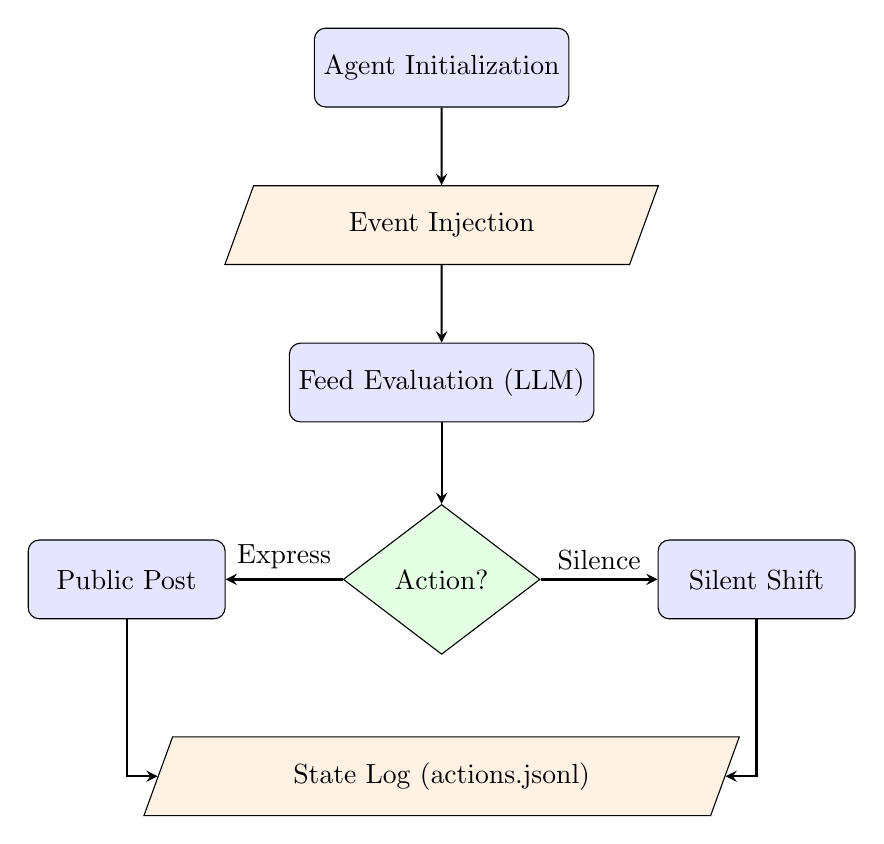
\begin{tikzpicture}[node distance=1.5cm, auto]
\tikzstyle{process} = [rectangle, minimum width=2.5cm, minimum height=1cm, text centered, draw=black, fill=blue!10, rounded corners]
\tikzstyle{io} = [trapezium, trapezium left angle=70, trapezium right angle=110, minimum width=2cm, minimum height=1cm, text centered, draw=black, fill=orange!10]
\tikzstyle{decision} = [diamond, minimum width=2.5cm, minimum height=1cm, text centered, draw=black, fill=green!10]
\tikzstyle{arrow} = [thick,->,>=stealth]

\node (init) [process] {Agent Initialization};
\node (event) [io, below of=init, yshift=-0.5cm] {Event Injection};
\node (feed) [process, below of=event, yshift=-0.5cm] {Feed Evaluation (LLM)};
\node (decision) [decision, below of=feed, yshift=-1cm] {Action?};
\node (public) [process, left of=decision, xshift=-2.5cm] {Public Post};
\node (silent) [process, right of=decision, xshift=2.5cm] {Silent Shift};
\node (log) [io, below of=decision, yshift=-1cm] {State Log (actions.jsonl)};

\draw [arrow] (init) -- (event);
\draw [arrow] (event) -- (feed);
\draw [arrow] (feed) -- (decision);
\draw [arrow] (decision) -- node[anchor=south] {Express} (public);
\draw [arrow] (decision) -- node[anchor=south] {Silence} (silent);
\draw [arrow] (public) |- (log);
\draw [arrow] (silent) |- (log);
\end{tikzpicture}
\caption{MiroFish Pipeline Workflow Diagram}
\label{fig:pipeline}
\end{figure}

The public action outcomes include:
\begin{itemize}
    \item \textbf{Supportive/Opposing Post}: Publicly expressing their stance.
    \item \textbf{Silent Shift / No Action}: Choosing to remain silent despite being exposed to the information, often due to high social pressure or fear.
\end{itemize}

\subsection{Live Polling and Aggregation}
A critical technical challenge in ABM is the real-time aggregation of thousands of agent states. The MiroFish backend employs a high-performance polling mechanism that parses the event log (`actions.jsonl`) to compute cumulative and instantaneous metrics.

\section{Core Contributions}

\subsection{Quantifying Preference Falsification}
The platform distinctively tracks both the private stance (`private_stance`) and the public action of every agent. By comparing these variables, the system computes the Preference Falsification gap. For instance, if an agent possesses a "Supporting" true stance but outputs a "Silent Shift" action, they are classified as expressing a "Neutral" public stance. This gap is visualized in real-time, providing immediate insights into silent majorities.

\subsection{Campaign Reach and Visibility Tracking}
Traditional engagement metrics only track visible interactions (likes, shares, posts). MiroFish introduces a tri-state visibility model:
\begin{enumerate}
    \item \textbf{Expressed}: Agents who saw the campaign and engaged publicly.
    \item \textbf{Silent}: Agents who were exposed to the campaign but chose not to act.
    \item \textbf{Unaware}: Agents who have not yet encountered the campaign in their feed.
\end{enumerate}
By tracking the cumulative exposure sets across all simulation rounds, campaign managers can accurately assess the true reach of their messaging, including the "dark reach" of silent observers.

\section{Conclusion and Future Work}
MiroFish represents a significant step forward in applied computational social science, offering a granular, real-time window into complex social dynamics like preference falsification. Future iterations of the system will focus on integrating more advanced LLM reasoning capabilities and expanding the network topology to model cross-platform information flows (e.g., between X/Twitter and Reddit).

\bibliographystyle{IEEEtran}
\begin{thebibliography}{00}
\bibitem{kuran1995private}
T.~Kuran, \textit{Private Truths, Public Lies: The Social Consequences of Preference Falsification}. Harvard University Press, 1995.
\end{thebibliography}

\end{document}
